\begin{LQ}{Modèle de l'environnement}

\LQDescription{
    Le modèle de l'environnement décrit les messages entre le système et les
    acteurs son environnement. Les acteurs sont par exemple des actionneurs
    (boutons, leviers, capteurs, ...) ou des vecteurs d'informations (témoins
    lumineux, affichage digital, écran, ...). Le système apparaît lui même comme
    une boîte noire où seules les interactions apparaissent.
}

\LQSchema{

Un peu sur le même principe que pour les schéma du CdU, ceux du MdE sont composés du système/sous-système, d’acteur de leurs actions respectives. Le système en “boite noire” est représenté par un rectangle avec le nom du système en titre. Les différentes acteurs sont représentés par des bon-hommes et relié au système par des traits pleins. Les différentes actions entre le système et un acteur sont décrits au dessus d’une flèche que le dialogue se fasse du système vers le dialogue ou l’inverse. Pour finir,on utilisera un astérisque (*) pour signifier qu’un acteur est présent plusieurs fois dans le système.

}

\begin{figure}
   \centering
   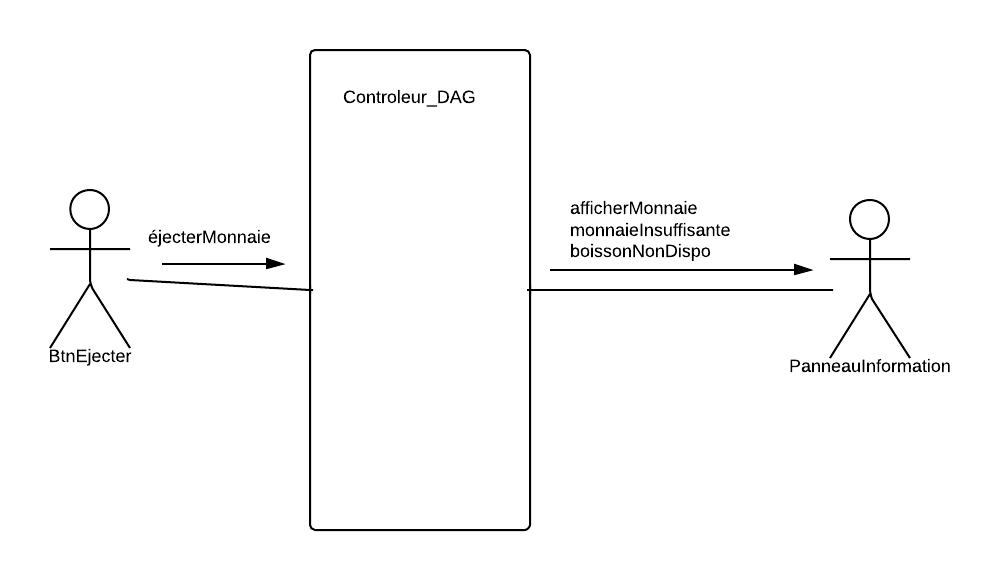
\includegraphics[width=\textwidth]{../images/MdE.png}
   \caption{Schéma du modèle de l'environnement}
\end{figure}


\LQModel{
    Chaque MdE correspond un sous-système qui découle de l'analyse des
    différents CdU. \\

    Les acteurs du MdE communiquent et échangent des messages avec le système
    étudié. Ils sont différents de ceux des CdU. Il sont intermédiaire direct.
    entre un acteur du CdU et le système (le bouton est l'intermédiaire direct
    entre le consommateur et le système "distributeur automatique"). Cependant,
    il est possible que les deux acteurs soient confondus dans certains cas.
    Nous essayerons au mieux de différencier les acteurs du CdU et de la MdE. \\

    A une action de l'environnement vers le système, doit correspondre une
    action d'un utilisateur vers le système dans le Cdu (et inversement).
    L'action "afficherMonnaie" que reçoit l'acteur "PanneauInformation" découle
    du cas d'utilisation "acheterBoisson". Plus le scénario d'un cas
    d'utilisation est précis, plus les MdE sont simples à concevoir.
}

\LQBetweenModels{
Lorsqu'il existe plusieurs modèle de l'environnement différent pour une même structure, il faut s'assurer de la cohérence entre ces modèles. Ainsi si il existe un échange de message entre un  système et un acteur dans un modèles de l'environnement, il faut s'assurer que cette échange de message reste le même dans un autre modèle.
}

\end{LQ}
